%%%%%%%%%%%%%%%%%%%%%%%%%%%%%%%%%%%%%%%%%%%%%%%%%%%%%%%%%%%%%%%%%%%%%%%%%%%%%%%%%%%%%%%%%
% SECTION HYDRODYNAMIC SIMULATIONS 
%%%%%%%%%%%%%%%%%%%%%%%%%%%%%%%%%%%%%%%%%%%%%%%%%%%%%%%%%%%%%%%%%%%%%%%%%%%%%%%%%%%%%%%%%

\section{Hydrodynamic Simulations}
\subsection{Code Description}

The code we used is called SLH (Seven League Hydro). It was originally developed by Dr. Fabian Miczek (2013) during his PhD thesis. SLH is a finite-volume multidimentional code that solves Euler equations (Ideal Hydrodynamic) using explicit or implicit methods. The advantage of implicit methos lies in the fact that the time step is constantly redefined optimizing computational resources using the so called CFL criterion for numerical stability. In this case a non-linear system of equations is solved using the Newton-Ralphson method, in which at every time step a linear system is solved through the Krylov subspace methods. The efficiency of all these computational methods is strongly dependent on the type of linear system solved and the cluster architecture used. \\
From the point of view of simulation domain SLH allows to implement a general curvilinear grid instead of a simple cartesian one by defining a metric, the elements of which are needed to correctly compute the fluxes at the cells interfaces. The code decomposes automatically the domain to parallelize the computation on the desired number of processors, using MPI and openMP. A wide choiche of boundary conditions are offered. \\
Furthermore SLH implements a general equation of state, a Nuclear Reaction Network, passive and active scalar which are fundamental for the study of the chemical composition of the fluid, radiation in the diffusion limit and thermal conduction. \\
Over the years SHL has undergone several scaling tests, the most remarkalbe of which at the Julich Computing Center in 2016 where it scaled over all the $458752$ cores of \textit{JUQUEEN} (a Blue Gene machine, currently the last generation of IBM supercomputers).
\subsection{2D Simulations}
\subsubsection{Simulations setup}
The physical setup used for our simulations is the so called "box in a star" method, meaning that we simulate some very small internal region of a star. \\
In our case for the 2D runs it will be a box of $2.50 \times 10^{9} cm$ on the $x$ axis and $1.25 \times 10^{9} cm$ on the $y$ axis. Gravity is constant pointing downward on the $y$ axis with a magnitude of $1000 cm/s^2$. This generates a pressure statification in the fluid that covers approximately three pressure scale heigh. \\
\begin{figure}[t]
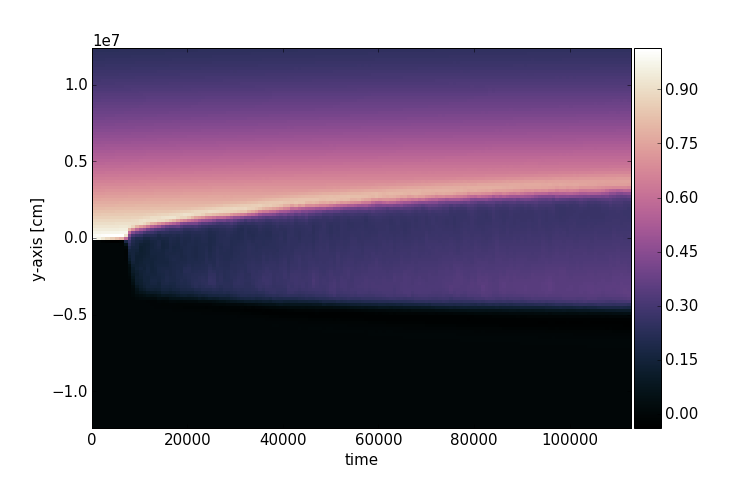
\includegraphics[width=10cm]{./img/tempprofile}
\caption{Example of initial temperature profile along the $y$-axis}
\label{fig:tempprofile}
\centering
\end{figure}
The controlling parameter is the temperature gradient that can we initialized to any value. In our case we divided the simulated region in three parts. The bottom region (labeled as $1$) starts at the lower boundary and reaches $4/12$ of the domain, the central (labeled as $2$) proceeds till the middle, and the upper one (labeled as $3$) reaches the upper boundary, as shown in \ref{fig:tempprofile}. We define a parameter $\alpha_{i}$ ($i=1, 2, 3$) which is nothing but the fraction of the $\nabla$ over the $\nabla_{\mathrm{ad}}$. As seen in previous sections $\alpha_{i}<1$ implies stability in the $i-$region, instability otherwise. \\
\begin{figure}[t]
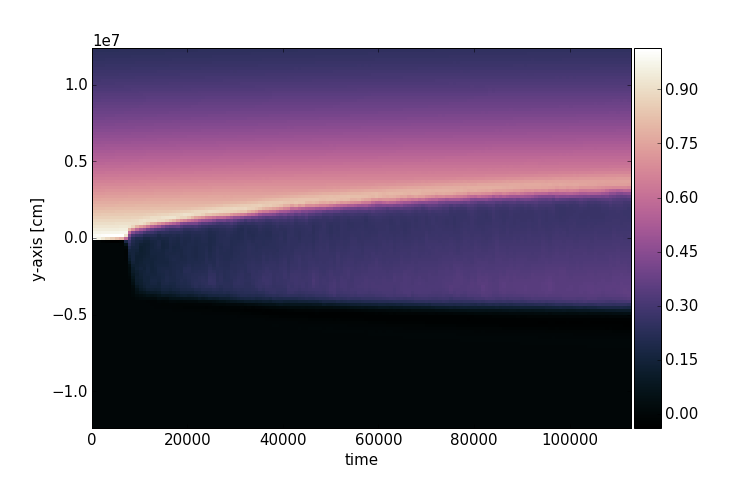
\includegraphics[width=10cm]{./img/tempprofile}
\caption{Example of initial temperature profile along the $y$-axis}
\label{fig:tempprofile}
\centering
\end{figure}
We always initialized the setup with $\alpha_{1} = \alpha_{3}$ widely smaller than $1$; and $\alpha_{2}=0.99$, which means a very precarious situation in terms of stability in the second region. A heating function furthermore heats the second region with a gaussian profile (see \label{fig:tempprofile}) to generate convection that will expand downward and upward by accretion. The values of $\alpha_{1}$ and $\alpha_{3}$ are controlling parameters for the bulk-Richardson number, since they are proportional to $\Delta b$. The advantage of simulating a strip of convection between two stable layers (miming a Shell convection) instead of a convective region at the bottom that grows upward (Core convection-like) is twofold: it gives us two convective boundaries to study instead of one, and we avoid high mach number at the boundary which can at times generate problems or unphysical situations. \\
One of the hardest tasks has been to generate the correct amount of heating such that the turbulence route mean square \textit{at the interface} was constant during the run (which is one one of the ingredients of the bulk-Richardson number, hence one of the parameters we want to control in order to perform a differential study). The heating function also checks at every time step if in any cell of the grid a given mach number limit is reached. In that case the total heating is reduced to $50 \%$ of the original amount.\\ 
At the bottom of the simulated region small perturbations in temperature and mach number had been imprinted on the stratification in order to break the initial symmetry of the system.\\
A wide range of boundary condition has been tested for this problem. Periodic boundaries along the $y$-axis would have provided the most physical solution, unfortunately an horizontal shear flow used to appear at the onset of convection. We observed the same shear flow using boundary with constant extrapolation for the velocity field. Eventually we decided to use wall boundary conditions everywhere. \\
As briefly explained in the previous sections, in order to define the topology of the convective boundaries, we injected a passive scalar inside the central region. Recall that passive scalars are just like colors of the fluid and in no way they influence the dynamic of the system, neither they diffuse.\\
As previously stated our goal is to perform a \textit{differential} study of the bulk-richardson number and the CBM problem. This implies running simulations with different values of $\Delta b$ and $\sigma_t$ at different resolutions. Being 2D simulations computationally speaking so cheap we managed to run a copious amount of them. As reported in ??? we run with $\alpha_1=\alpha_3=0.2, 0.7$, mach number limit of $0.5, 0.01$, and resolution spanning from $256 \times 128$ (Low Resolution, LR), $512 \times 256$ (MR), $1024 \times 512$ (HR), $2048 \times 1024$ (VR). With this notation with the code 2d0.7-0.01HR we refer to a 2 dimensional simulation, with $\alpha_1=\alpha_3=0.7$, a reduction of the heating at mach $0.01$ on a $1024 \times 512$ grid. \\
It is worth noticing that a higher resolution in CFD does not only mean resolving better the system, but also changing the numerical viscosity of the fluid. Hence we expect to have higher mach number on higher resolution runs.
Numerical viscosity is also the reason for which on the $x$-axis the number of cells is always the double to the $y$-axis: we want to keep cells squared and not rectangular, in order to keep viscosity isotropic and prevent it from becoming a tensorial quantity. \\

\subsubsection{Evolution of a single run}
Let's consider the setup 2d0.7-0.01LR. \\
Convection starts at around $t \sim 7000 s$. Because of the already mentioned implicit time stepping, the lower the mach number, the bigger the time step, allowing us to save a huge amount of computational resources before the rise of convection. A remarkable difference is also observed in the convective regime, as long as the mach number is below $10 \%$, which will always be our case. \\
In figure \ref{fig:2d0.7-0.01LR.passive} we plot the passive scalar (initialized inside the central region) which over time is advected by convection. We clearly see the accretion of the convective boundary that over the $200000 s$ of simulated time moves gradually upward and downward. Specifically in the upper case it starts at $\sim 6.2 \times 10^{6} cm $ and ends up at $\sim 8.0 \times 10^{6} cm$, for the lower case it starts at $\sim 3.7 \times 10^{6} cm$ and moves downwards to $\sim 3.1 \times 10^{6} cm$. \\
In figure \ref{fig:2d0.7-0.01LR.mach} we plot profile of the mach number over the simulated time. It is what one would expect by looking at the passive scalar adcevtion, with two remarks that need to be done. \\
First of all the mach number slightly grows over time but not dramaticaly, thanks to the heating function that we implemented, featuring a cutoff as previously explained. \\
Second of all it is clear that some internal modes are excited by the convective blobs when they hit the stable layers and they propagate through it. They appear more significative in the upper region and to a certain extent it's true, but mainly this is due to the fact that the speed of sound there it's lower. Plotting the absolute velocity the difference is not so dramatic. An intresting question why will try to answer to is obviously to which extent these internal modes influence the dynamic of the boundary. \\
\begin{figure}[t]
  \centering
    \subfloat[Advection of passive scalar and convective boundary growth]{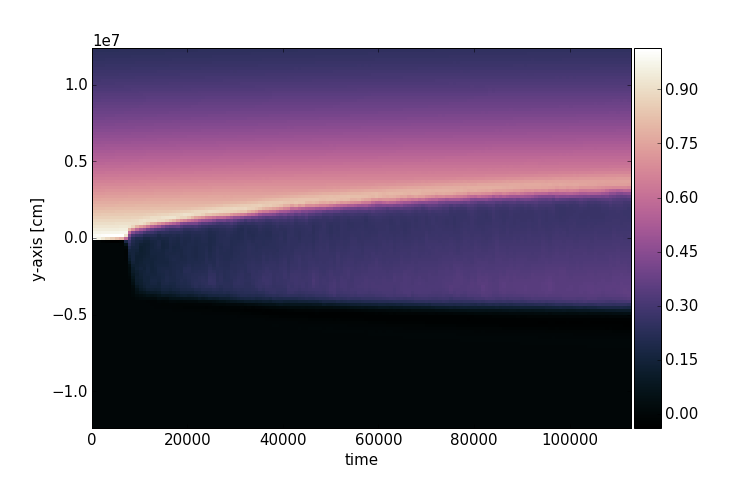
\includegraphics[width=0.4\textwidth]{./img/tempprofile}\label{fig:2d0.7-0.01LR.passive}}
      \hfill
        \subfloat[Profile of the mach number over time]{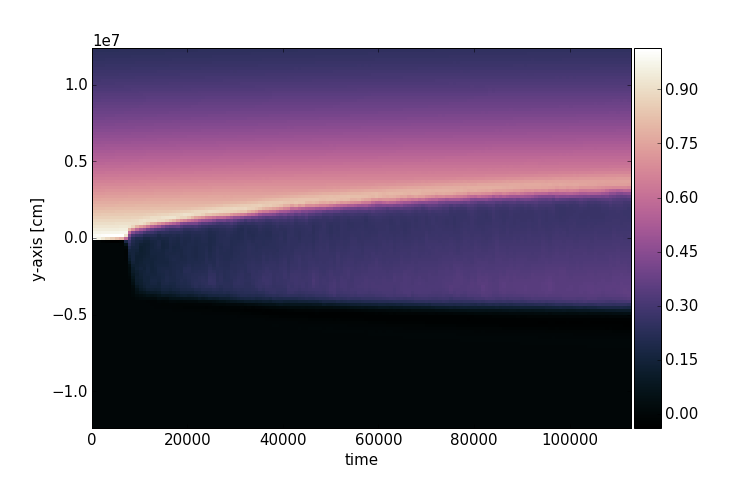
\includegraphics[width=0.4\textwidth]{./img/tempprofile}\label{fig:2d0.7-0.01LR.mach}}
	  \label{2d0.7-0.01LR.passive}
  \end{figure}
In figure \ref{fig:2d0.7-0.01LR.bp} we plot the parameters needed to compute the bulk-Richardson number for the upper boundary. \\
We show first of all the boundary position over time with its rms. It's clear that after $t \sim 100000 s$ there is a slow down, and we suspect that this is due to the interaction with the internal modes. \\
Second of all we plot in figure \ref{fig:2d0.7-0.01LR.turbmach} the turbulence rms mach number at the interface. This is not constant over the run, instead it oscillates, but we are satisfied by the fact that it remains in the same order of magnitude. There is also a tiny trend to increase, but as previously stated, it is an extremely hard task to tune the heating in order to obtain a perfectly constant turbulent regime. \\
\begin{figure}[t]
  \centering
    \subfloat[Advection of passive scalar and convective boundary growth]{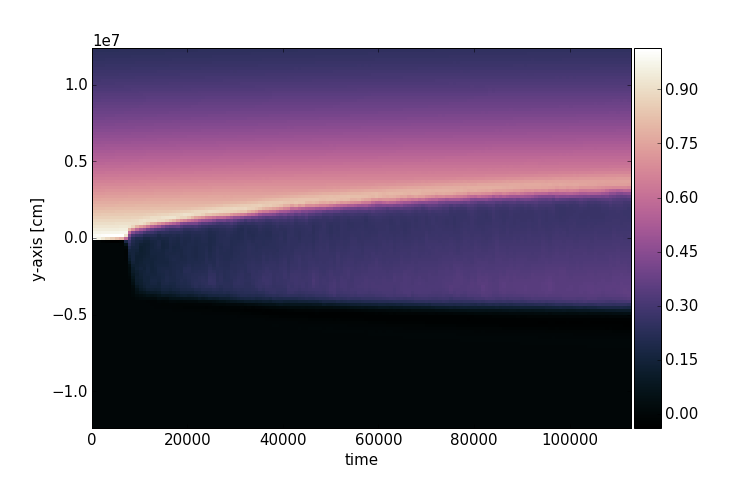
\includegraphics[width=0.4\textwidth]{./img/tempprofile}\label{fig:2d0.7-0.01LR.bp}}
      \hfill
        \subfloat[Profile of the mach number over time]{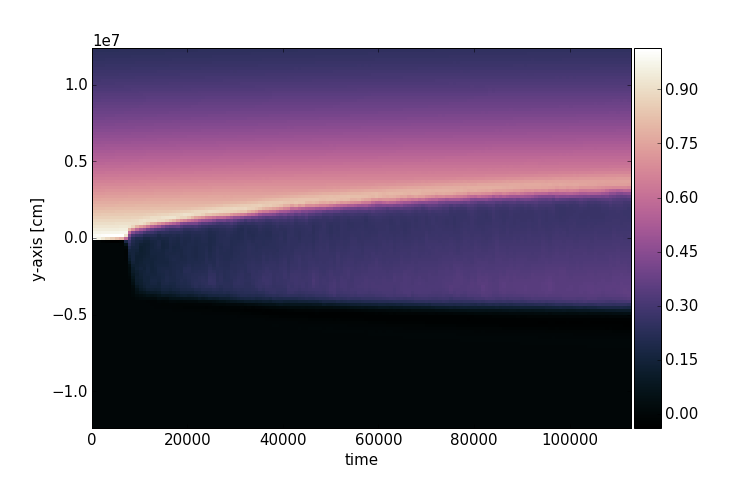
\includegraphics[width=0.4\textwidth]{./img/tempprofile}\label{fig:2d0.7-0.01LR.turbmach}}
      \hfill
        \subfloat[Profile of the mach number over time]{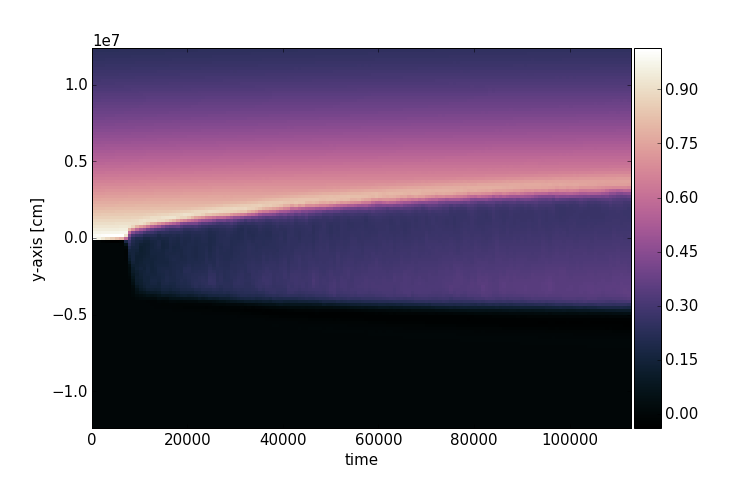
\includegraphics[width=0.4\textwidth]{./img/tempprofile}\label{fig:2d0.7-0.01LR.delb}}
      \hfill
        \subfloat[Profile of the mach number over time]{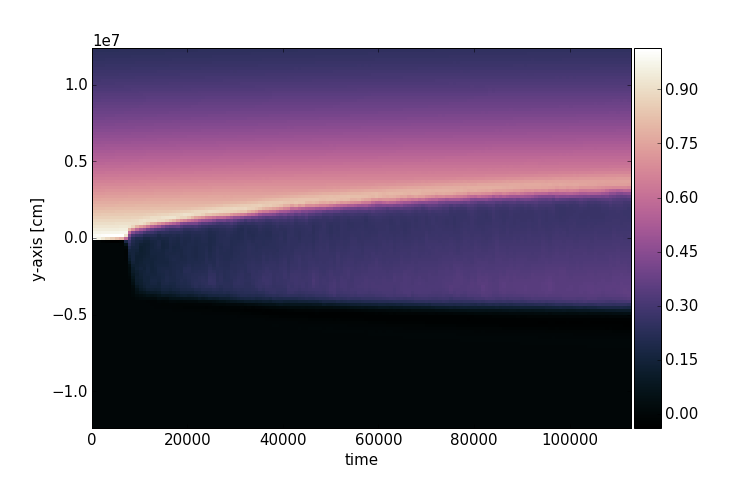
\includegraphics[width=0.4\textwidth]{./img/tempprofile}\label{fig:2d0.7-0.01LR.l}}
	\caption{prova caption}
  \end{figure}
In figure \ref{fig:2d0.7-0.01LR.delb} we plot the buoyancy jump acros the interface. By looking at this it is clear that the resolution used in this run is absolutely not enough to properly resolve the system. As previously explained the $\Delta b$ is obtained by integrating the Brunt-Väsälä frequency over the boundary rms, but in some cases this is less than half of a cell, hence when discretized it goes down to zero. This is the reason for which we get a plot with such discontinuities. As we will see, this inconvenient will not occur anymore with higher resolution runs. \\
Last we plot in figure \ref{fig:2d0.7-0.01LR.l} the turbulence length scale. This is computed by autocorrelating the mach number at the center of the convective region, and then taking the length at which the autocorrelation function drops below $0.5$. It is remarkable that this parameter oscillates very much over a full order of magnitude, but does not show any increasing or decreasing trend. We decided to compute it in the middle of the region, rather than on the boundary, because in the second case the magnitude of the oscillation was too high and impracticable. \\
For every 2D or 3D run we will extrapolate the relevant parameters and present in the following layout
\begin{center}
 \begin{tabular}{|l|c|c|c|c|c|c|}
	  \hline
	  Run & $\Delta b$ & $\sigma_t$ & $L$ & $Ri_{\mathrm{B}}$ & $u_E$ & exp vel\\
	  	\hline
		2d0.7-0.01LR & 5 & 7& 5 & 7& 5 & 7 \\ 
	      \hline
      \end{tabular}
 \end{center}

\subsubsection{Resolution study}
The previous LR case is the lowest resolution we can use to compute the buoyancy jump. The reason is that when using a $128 \times 64$ grid, the boundary width is at times below half of a cell (which is consequentially rounded down to zero), leading to $\Delta b =0$. Once the resolution is enhanced at the point that the bouyancy jump is always nonzero, still this does not imply that we are properly resolving all the features of the system relevant to our problem, like smaller turbulent blobs that might have an impact on the CBM. For this reason we run the previous setup at different resolution, and we are going to discuss the results in the following paragraphs.

